\subsection{Unit Step and Dirac Delta Distribution}
\subsubsection{Unit step function}
\begin{figure}[H]
    \centering
    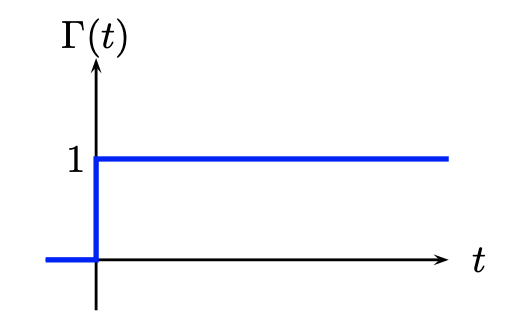
\includegraphics[scale=0.6]{figures/unit_step_func.png}
    \caption{The unit step- or Heaviside function}
    \label{fig:unit_step_function}
\end{figure}

The unit step function or Heaviside function is defined by:
\begin{align*}
\Gamma(t) =
    \begin{cases}
    0,& t<0\\
    \dfrac{1}{2}, & t=0\\
    1, & t>0
\end{cases}.
\end{align*}


\noindent The unit step function has the following relation with the Dirac Delta function
\begin{align*}
 u(t)=\int_{-\infty}^{t}\delta(\tau)d\tau. 
\end{align*}


\subsubsection{Dirac Delta}
\begin{definition}{The Dirac Delta Distribution} \label{DiracDeltaDef}
The Dirac Delta distribution is a map $\delta : \mathbb{R} \rightarrow \mathbb{R} \cup \{\infty\}$, which yealds zero everywhere execpt at the origin, where it is infinte:

\begin{align*}
\delta(t) =
    \begin{cases}
    +\infty,& t=0\\
    0, & t \neq 0
\end{cases},
\end{align*}
and satisfies the identity
\begin{align*}
    \int_{-\infty}^{\infty} f(t) \delta(t) dt = f(0)
\end{align*}
for any $f: \mathbb{R} \rightarrow \mathbb{R}$ bounded and continuous at $t=0$.
\end{definition}

%skal vi have en graf med, der viser den?

Futhermore $\delta(t)$, which will be referred to as the unit impulse, has the following properties:
\begin{enumerate}
    \item $\delta(t) \rightarrow \infty \; as \; t \rightarrow 0$
    \item $\delta(t) =0 \; for \; t \neq 0$
    \item $\int_{-\infty}^{\infty} \delta(t) dt =1$
    \item $\delta(t)= \delta(-t)$
\end{enumerate}

\noindent The unit impulse also has a property called the sifting property, which is expressed by:

\begin{align*}
\int_{t_1}^{t_2} y(t) \delta(t-t_0)dt = 
    \begin{cases}
    y(t_0),& t_1<t_0<t_2\\
    0, & \text{otherwise}
\end{cases},
\end{align*}
where $y(t)$ is an $\mathcal{L}_2$ function. This is achieved by changing the variables to $\tau =t$ and inserting this in \autoref{DiracDeltaDef}.\cite{LectureNotes}
